\documentclass[]{article}
\usepackage{lmodern}
\usepackage{amssymb,amsmath}
\usepackage{ifxetex,ifluatex}
\usepackage{fixltx2e} % provides \textsubscript
\ifnum 0\ifxetex 1\fi\ifluatex 1\fi=0 % if pdftex
  \usepackage[T1]{fontenc}
  \usepackage[utf8]{inputenc}
\else % if luatex or xelatex
  \ifxetex
    \usepackage{mathspec}
  \else
    \usepackage{fontspec}
  \fi
  \defaultfontfeatures{Ligatures=TeX,Scale=MatchLowercase}
\fi
% use upquote if available, for straight quotes in verbatim environments
\IfFileExists{upquote.sty}{\usepackage{upquote}}{}
% use microtype if available
\IfFileExists{microtype.sty}{%
\usepackage{microtype}
\UseMicrotypeSet[protrusion]{basicmath} % disable protrusion for tt fonts
}{}
\usepackage[margin=1in]{geometry}
\usepackage{hyperref}
\hypersetup{unicode=true,
            pdftitle={R Notebook},
            pdfauthor={Sanne Meijering; Hanne Oberman; Gerbrich Ferdinands},
            pdfborder={0 0 0},
            breaklinks=true}
\urlstyle{same}  % don't use monospace font for urls
\usepackage{color}
\usepackage{fancyvrb}
\newcommand{\VerbBar}{|}
\newcommand{\VERB}{\Verb[commandchars=\\\{\}]}
\DefineVerbatimEnvironment{Highlighting}{Verbatim}{commandchars=\\\{\}}
% Add ',fontsize=\small' for more characters per line
\usepackage{framed}
\definecolor{shadecolor}{RGB}{248,248,248}
\newenvironment{Shaded}{\begin{snugshade}}{\end{snugshade}}
\newcommand{\KeywordTok}[1]{\textcolor[rgb]{0.13,0.29,0.53}{\textbf{{#1}}}}
\newcommand{\DataTypeTok}[1]{\textcolor[rgb]{0.13,0.29,0.53}{{#1}}}
\newcommand{\DecValTok}[1]{\textcolor[rgb]{0.00,0.00,0.81}{{#1}}}
\newcommand{\BaseNTok}[1]{\textcolor[rgb]{0.00,0.00,0.81}{{#1}}}
\newcommand{\FloatTok}[1]{\textcolor[rgb]{0.00,0.00,0.81}{{#1}}}
\newcommand{\ConstantTok}[1]{\textcolor[rgb]{0.00,0.00,0.00}{{#1}}}
\newcommand{\CharTok}[1]{\textcolor[rgb]{0.31,0.60,0.02}{{#1}}}
\newcommand{\SpecialCharTok}[1]{\textcolor[rgb]{0.00,0.00,0.00}{{#1}}}
\newcommand{\StringTok}[1]{\textcolor[rgb]{0.31,0.60,0.02}{{#1}}}
\newcommand{\VerbatimStringTok}[1]{\textcolor[rgb]{0.31,0.60,0.02}{{#1}}}
\newcommand{\SpecialStringTok}[1]{\textcolor[rgb]{0.31,0.60,0.02}{{#1}}}
\newcommand{\ImportTok}[1]{{#1}}
\newcommand{\CommentTok}[1]{\textcolor[rgb]{0.56,0.35,0.01}{\textit{{#1}}}}
\newcommand{\DocumentationTok}[1]{\textcolor[rgb]{0.56,0.35,0.01}{\textbf{\textit{{#1}}}}}
\newcommand{\AnnotationTok}[1]{\textcolor[rgb]{0.56,0.35,0.01}{\textbf{\textit{{#1}}}}}
\newcommand{\CommentVarTok}[1]{\textcolor[rgb]{0.56,0.35,0.01}{\textbf{\textit{{#1}}}}}
\newcommand{\OtherTok}[1]{\textcolor[rgb]{0.56,0.35,0.01}{{#1}}}
\newcommand{\FunctionTok}[1]{\textcolor[rgb]{0.00,0.00,0.00}{{#1}}}
\newcommand{\VariableTok}[1]{\textcolor[rgb]{0.00,0.00,0.00}{{#1}}}
\newcommand{\ControlFlowTok}[1]{\textcolor[rgb]{0.13,0.29,0.53}{\textbf{{#1}}}}
\newcommand{\OperatorTok}[1]{\textcolor[rgb]{0.81,0.36,0.00}{\textbf{{#1}}}}
\newcommand{\BuiltInTok}[1]{{#1}}
\newcommand{\ExtensionTok}[1]{{#1}}
\newcommand{\PreprocessorTok}[1]{\textcolor[rgb]{0.56,0.35,0.01}{\textit{{#1}}}}
\newcommand{\AttributeTok}[1]{\textcolor[rgb]{0.77,0.63,0.00}{{#1}}}
\newcommand{\RegionMarkerTok}[1]{{#1}}
\newcommand{\InformationTok}[1]{\textcolor[rgb]{0.56,0.35,0.01}{\textbf{\textit{{#1}}}}}
\newcommand{\WarningTok}[1]{\textcolor[rgb]{0.56,0.35,0.01}{\textbf{\textit{{#1}}}}}
\newcommand{\AlertTok}[1]{\textcolor[rgb]{0.94,0.16,0.16}{{#1}}}
\newcommand{\ErrorTok}[1]{\textcolor[rgb]{0.64,0.00,0.00}{\textbf{{#1}}}}
\newcommand{\NormalTok}[1]{{#1}}
\usepackage{graphicx,grffile}
\makeatletter
\def\maxwidth{\ifdim\Gin@nat@width>\linewidth\linewidth\else\Gin@nat@width\fi}
\def\maxheight{\ifdim\Gin@nat@height>\textheight\textheight\else\Gin@nat@height\fi}
\makeatother
% Scale images if necessary, so that they will not overflow the page
% margins by default, and it is still possible to overwrite the defaults
% using explicit options in \includegraphics[width, height, ...]{}
\setkeys{Gin}{width=\maxwidth,height=\maxheight,keepaspectratio}
\IfFileExists{parskip.sty}{%
\usepackage{parskip}
}{% else
\setlength{\parindent}{0pt}
\setlength{\parskip}{6pt plus 2pt minus 1pt}
}
\setlength{\emergencystretch}{3em}  % prevent overfull lines
\providecommand{\tightlist}{%
  \setlength{\itemsep}{0pt}\setlength{\parskip}{0pt}}
\setcounter{secnumdepth}{0}
% Redefines (sub)paragraphs to behave more like sections
\ifx\paragraph\undefined\else
\let\oldparagraph\paragraph
\renewcommand{\paragraph}[1]{\oldparagraph{#1}\mbox{}}
\fi
\ifx\subparagraph\undefined\else
\let\oldsubparagraph\subparagraph
\renewcommand{\subparagraph}[1]{\oldsubparagraph{#1}\mbox{}}
\fi

%%% Use protect on footnotes to avoid problems with footnotes in titles
\let\rmarkdownfootnote\footnote%
\def\footnote{\protect\rmarkdownfootnote}

%%% Change title format to be more compact
\usepackage{titling}

% Create subtitle command for use in maketitle
\newcommand{\subtitle}[1]{
  \posttitle{
    \begin{center}\large#1\end{center}
    }
}

\setlength{\droptitle}{-2em}
  \title{R Notebook}
  \pretitle{\vspace{\droptitle}\centering\huge}
  \posttitle{\par}
  \author{Sanne Meijering \\ Hanne Oberman \\ Gerbrich Ferdinands}
  \preauthor{\centering\large\emph}
  \postauthor{\par}
  \date{}
  \predate{}\postdate{}


\begin{document}
\maketitle

\section{Initialization}\label{initialization}

\begin{Shaded}
\begin{Highlighting}[]
\CommentTok{# Load packages}
\KeywordTok{require}\NormalTok{(survey)}
\end{Highlighting}
\end{Shaded}

\begin{verbatim}
## Loading required package: survey
\end{verbatim}

\begin{verbatim}
## Warning: package 'survey' was built under R version 3.4.4
\end{verbatim}

\begin{verbatim}
## Loading required package: grid
\end{verbatim}

\begin{verbatim}
## Loading required package: Matrix
\end{verbatim}

\begin{verbatim}
## Loading required package: survival
\end{verbatim}

\begin{verbatim}
## 
## Attaching package: 'survey'
\end{verbatim}

\begin{verbatim}
## The following object is masked from 'package:graphics':
## 
##     dotchart
\end{verbatim}

\begin{Shaded}
\begin{Highlighting}[]
\KeywordTok{require}\NormalTok{(sampling)}
\end{Highlighting}
\end{Shaded}

\begin{verbatim}
## Loading required package: sampling
\end{verbatim}

\begin{verbatim}
## Warning: package 'sampling' was built under R version 3.4.4
\end{verbatim}

\begin{verbatim}
## 
## Attaching package: 'sampling'
\end{verbatim}

\begin{verbatim}
## The following objects are masked from 'package:survival':
## 
##     cluster, strata
\end{verbatim}

\begin{Shaded}
\begin{Highlighting}[]
\CommentTok{# Load society dataset}
\NormalTok{society <-}\StringTok{ }\KeywordTok{readRDS}\NormalTok{(}\StringTok{"Understanding Society innovation pnel wave A.RDS"}\NormalTok{)}
\NormalTok{society$a_dvage <-}\StringTok{ }\KeywordTok{as.numeric}\NormalTok{(society$a_dvage)}
\end{Highlighting}
\end{Shaded}

\section{Sampling design}\label{sampling-design}

\subsection{Question 2}\label{question-2}

Investigation of design weights

\begin{Shaded}
\begin{Highlighting}[]
\CommentTok{# Calculate variance of design weight}
\NormalTok{Var <-}\StringTok{ }\KeywordTok{var}\NormalTok{(society$a_psnenip_xd)}
\CommentTok{# Combine variance with other descriptive statistics}
\NormalTok{Descr <-}\StringTok{ }\KeywordTok{cbind}\NormalTok{(}\KeywordTok{t}\NormalTok{(}\KeywordTok{summary}\NormalTok{(society$a_psnenip_xd)), Var)}
\CommentTok{# Print with up to 2 decimals}
\KeywordTok{round}\NormalTok{(Descr, }\DecValTok{2}\NormalTok{)}
\end{Highlighting}
\end{Shaded}

\begin{verbatim}
##      Min. 1st Qu. Median Mean 3rd Qu. Max.  Var
## [1,]    1       1      1 1.01       1    4 0.02
\end{verbatim}

\subsection{Question 3}\label{question-3}

\begin{Shaded}
\begin{Highlighting}[]
\CommentTok{# First, make the dataset smaller by removing unnecessary columns}
\NormalTok{society_3 <-}\StringTok{ }\NormalTok{society[,-}\KeywordTok{c}\NormalTok{(}\DecValTok{5}\NormalTok{:}\DecValTok{7}\NormalTok{,}\DecValTok{9}\NormalTok{:}\DecValTok{56}\NormalTok{,}\DecValTok{60}\NormalTok{:}\DecValTok{75}\NormalTok{,}\DecValTok{77}\NormalTok{:}\DecValTok{89}\NormalTok{)]}

\CommentTok{# Investigate levels of government office region variable}
\KeywordTok{levels}\NormalTok{(society_3$a_gor_dv)}
\end{Highlighting}
\end{Shaded}

\begin{verbatim}
##  [1] "missing"                  "north east"              
##  [3] "north west"               "yorkshire and the humber"
##  [5] "east midlands"            "west midlands"           
##  [7] "east of england"          "london"                  
##  [9] "south east"               "south west"              
## [11] "wales"                    "scotland"                
## [13] "northern ireland"
\end{verbatim}

\begin{Shaded}
\begin{Highlighting}[]
\KeywordTok{nrow}\NormalTok{(society_3[society_3$a_gor_dv ==}\StringTok{ "missing"}\NormalTok{,])}
\end{Highlighting}
\end{Shaded}

\begin{verbatim}
## [1] 0
\end{verbatim}

\begin{Shaded}
\begin{Highlighting}[]
\KeywordTok{nrow}\NormalTok{(society_3[society_3$a_gor_dv ==}\StringTok{ "northern ireland"}\NormalTok{,])}
\end{Highlighting}
\end{Shaded}

\begin{verbatim}
## [1] 0
\end{verbatim}

\begin{Shaded}
\begin{Highlighting}[]
\CommentTok{# None of the value are missing or northern ireland, so those can be ignored}

\CommentTok{# Create dummy variables for government office regions}
\NormalTok{society_3$NE <-}\StringTok{ }\NormalTok{society_3$a_gor_dv ==}\StringTok{ "north east"}
\NormalTok{society_3$NW <-}\StringTok{ }\NormalTok{society_3$a_gor_dv ==}\StringTok{ "north west"}
\NormalTok{society_3$Y <-}\StringTok{ }\NormalTok{society_3$a_gor_dv ==}\StringTok{ "yorkshire and the humber"}
\NormalTok{society_3$EM <-}\StringTok{ }\NormalTok{society_3$a_gor_dv ==}\StringTok{ "east midlands"}
\NormalTok{society_3$WM <-}\StringTok{ }\NormalTok{society_3$a_gor_dv ==}\StringTok{ "west midlands"}
\NormalTok{society_3$EOE <-}\StringTok{ }\NormalTok{society_3$a_gor_dv ==}\StringTok{ "east of england"}
\NormalTok{society_3$L <-}\StringTok{ }\NormalTok{society_3$a_gor_dv ==}\StringTok{ "london"}
\NormalTok{society_3$SE <-}\StringTok{ }\NormalTok{society_3$a_gor_dv ==}\StringTok{ "south east"}
\NormalTok{society_3$SW <-}\StringTok{ }\NormalTok{society_3$a_gor_dv ==}\StringTok{ "south west"}
\NormalTok{society_3$W <-}\StringTok{ }\NormalTok{society_3$a_gor_dv ==}\StringTok{ "wales"}
\NormalTok{society_3$S <-}\StringTok{ }\NormalTok{society_3$a_gor_dv ==}\StringTok{ "scotland"}

\CommentTok{# Run linear regression (Scotland is the baseline for government office region)}
\NormalTok{coeff <-}\StringTok{ }\KeywordTok{with}\NormalTok{(society_3, }\KeywordTok{lm}\NormalTok{(a_psnenip_xw ~}\StringTok{ }\NormalTok{a_psnenip_xd +}\StringTok{ }\NormalTok{a_sex +}\StringTok{ }\NormalTok{a_dvage +}\StringTok{ }\NormalTok{NE +}\StringTok{ }\NormalTok{NW +}\StringTok{ }\NormalTok{Y}
                            \NormalTok{+}\StringTok{ }\NormalTok{EM +}\StringTok{ }\NormalTok{WM +}\StringTok{ }\NormalTok{EOE +}\StringTok{ }\NormalTok{L +}\StringTok{ }\NormalTok{SE +}\StringTok{ }\NormalTok{SW +}\StringTok{ }\NormalTok{W))}

\CommentTok{# Get and sort coefficients}
\NormalTok{coeff <-}\StringTok{ }\NormalTok{coeff$coefficients}
\NormalTok{coeff.gor <-}\StringTok{ }\KeywordTok{sort}\NormalTok{(coeff[}\DecValTok{5}\NormalTok{:}\DecValTok{15}\NormalTok{])}

\CommentTok{# Plot coefficients}
\KeywordTok{plot}\NormalTok{(coeff.gor)}
\end{Highlighting}
\end{Shaded}

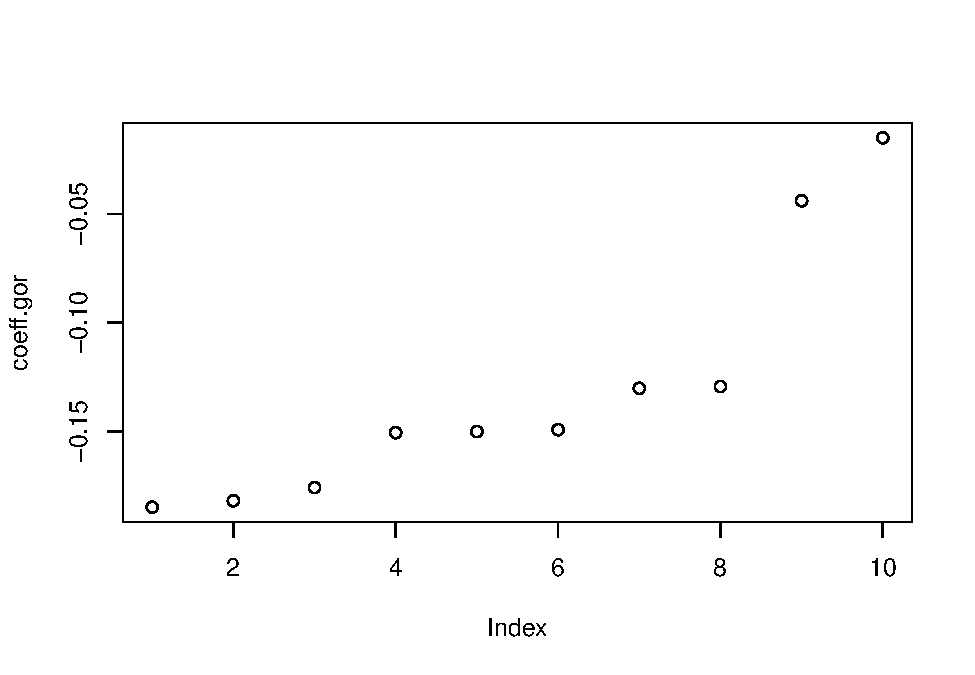
\includegraphics{SurveyFinalRcode_files/figure-latex/unnamed-chunk-3-1.pdf}

\begin{Shaded}
\begin{Highlighting}[]
\CommentTok{# Show coefficients}
\NormalTok{coeff.gor}
\end{Highlighting}
\end{Shaded}

\begin{verbatim}
##      SETRUE      NETRUE      SWTRUE       WTRUE       YTRUE      EMTRUE 
## -0.18484767 -0.18190941 -0.17581419 -0.15055368 -0.15005775 -0.14918625 
##     EOETRUE      NWTRUE      WMTRUE       LTRUE 
## -0.13013882 -0.12934118 -0.04394684 -0.01494428
\end{verbatim}

\section{Population Estimates}\label{population-estimates}

\subsection{Question 4}\label{question-4}

\begin{Shaded}
\begin{Highlighting}[]
\CommentTok{# Investigate the a_employ variable.}
\KeywordTok{levels}\NormalTok{(society$a_employ[society$a_dvage >}\StringTok{ }\DecValTok{15} \NormalTok{&}\StringTok{ }\NormalTok{society$a_dvage <}\StringTok{ }\DecValTok{64}\NormalTok{])}
\end{Highlighting}
\end{Shaded}

\begin{verbatim}
## [1] "missing"          "inapplicable"     "proxy respondent"
## [4] "refuse"           "don't know"       "yes"             
## [7] "no"
\end{verbatim}

\begin{Shaded}
\begin{Highlighting}[]
\CommentTok{# The variable a_employ has seven levels.}

\KeywordTok{summary}\NormalTok{(society$a_dvage[society$a_employ==}\StringTok{"yes"}\NormalTok{])}
\end{Highlighting}
\end{Shaded}

\begin{verbatim}
##    Min. 1st Qu.  Median    Mean 3rd Qu.    Max. 
##   22.00   38.00   48.00   47.55   57.00  102.00
\end{verbatim}

\begin{Shaded}
\begin{Highlighting}[]
\KeywordTok{summary}\NormalTok{(society$a_dvage[society$a_employ==}\StringTok{"no"}\NormalTok{])}
\end{Highlighting}
\end{Shaded}

\begin{verbatim}
##    Min. 1st Qu.  Median    Mean 3rd Qu.    Max. 
##   22.00   45.00   69.00   62.38   79.00  102.00
\end{verbatim}

\begin{Shaded}
\begin{Highlighting}[]
\CommentTok{# Yes and no contain people of over 21 years of age.}

\KeywordTok{nrow}\NormalTok{(society[society$a_employ==}\StringTok{"missing"}\NormalTok{,])}
\end{Highlighting}
\end{Shaded}

\begin{verbatim}
## [1] 0
\end{verbatim}

\begin{Shaded}
\begin{Highlighting}[]
\KeywordTok{nrow}\NormalTok{(society[society$a_employ==}\StringTok{"proxy respondent"}\NormalTok{,])}
\end{Highlighting}
\end{Shaded}

\begin{verbatim}
## [1] 0
\end{verbatim}

\begin{Shaded}
\begin{Highlighting}[]
\CommentTok{# Missing and proxy respondent do not appear in the data}

\KeywordTok{summary}\NormalTok{(society$a_dvage[society$a_employ==}\StringTok{"inapplicable"}\NormalTok{])}
\end{Highlighting}
\end{Shaded}

\begin{verbatim}
##    Min. 1st Qu.  Median    Mean 3rd Qu.    Max. 
##    6.00   10.00   14.00   13.79   18.00   21.00
\end{verbatim}

\begin{Shaded}
\begin{Highlighting}[]
\CommentTok{# Inapplicable seems to contain all children and youths of 21 years and younger}
\CommentTok{# It cannot be assumed that none of them is employed. It can however be assumed that only a}
\CommentTok{# small part of them is employed, as children under 15 cannot be employed legally}
\CommentTok{# and most would still be going to a school or university.}

\KeywordTok{nrow}\NormalTok{(society[society$a_employ==}\StringTok{"refuse"}\NormalTok{,])}
\end{Highlighting}
\end{Shaded}

\begin{verbatim}
## [1] 1
\end{verbatim}

\begin{Shaded}
\begin{Highlighting}[]
\KeywordTok{nrow}\NormalTok{(society[society$a_employ==}\StringTok{"don}\CharTok{\textbackslash{}'}\StringTok{t know"}\NormalTok{,])}
\end{Highlighting}
\end{Shaded}

\begin{verbatim}
## [1] 1
\end{verbatim}

\begin{Shaded}
\begin{Highlighting}[]
\CommentTok{# Both refuse and don't know contain one row. These can be treated as missing data.}

\CommentTok{# Thus, our goal is to compare the proportion of employed people (yes) of working age against }
\CommentTok{# the number of unemployed people (no, inapplicable), excluding the missing data (refuse, don't know)}

\KeywordTok{with}\NormalTok{(society, }\KeywordTok{nrow}\NormalTok{(society[a_employ==}\StringTok{"yes"} \NormalTok{&}\StringTok{ }\NormalTok{a_dvage >}\DecValTok{64}\NormalTok{,]))}
\end{Highlighting}
\end{Shaded}

\begin{verbatim}
## [1] 160
\end{verbatim}

\begin{Shaded}
\begin{Highlighting}[]
\CommentTok{# There are people older than 64 still working, we should exclude those. }
\KeywordTok{with}\NormalTok{(society, }\KeywordTok{nrow}\NormalTok{(society[a_employ==}\StringTok{"yes"} \NormalTok{&}\StringTok{ }\NormalTok{a_dvage <}\DecValTok{15}\NormalTok{,]))}
\end{Highlighting}
\end{Shaded}

\begin{verbatim}
## [1] 0
\end{verbatim}

\begin{Shaded}
\begin{Highlighting}[]
\CommentTok{# No one younger than 15 years is reported to be working, which is to be expected as it was not}
\CommentTok{# a question asked to people under 21 years of age.}

\CommentTok{# Since we wish to know the proportion of employed people of working age, we need 2 groups, one with employed adults and one with unemployed people and employed elderly.}
\NormalTok{society$employ_dv <-}\StringTok{ }\KeywordTok{as.numeric}\NormalTok{(}\DecValTok{0}\NormalTok{)}
\NormalTok{society$employ_dv[society$a_employ==}\StringTok{'yes'} \NormalTok{&}\StringTok{ }\NormalTok{society$a_dvage <=}\StringTok{ }\DecValTok{65}\NormalTok{] <-}\StringTok{ }\DecValTok{1}

\CommentTok{# Create design}
\CommentTok{# Don't remove the missing values yet, as the weights are calculated including missing values }
\NormalTok{Design <-}\StringTok{ }\KeywordTok{svydesign}\NormalTok{(}\DataTypeTok{ids=}\NormalTok{~a_hidp, }\DataTypeTok{strata=}\NormalTok{~a_strata, }\DataTypeTok{data=}\NormalTok{society, }\DataTypeTok{weights=}\NormalTok{~a_psnenip_xw)}
\CommentTok{# Make a subset of non-missing values}
\NormalTok{Nonmiss <-}\StringTok{ }\KeywordTok{with}\NormalTok{(Design, }\KeywordTok{subset}\NormalTok{(Design, a_employ!=}\StringTok{"refuse"} \NormalTok{&}\StringTok{ }\NormalTok{a_employ!=}\StringTok{"don}\CharTok{\textbackslash{}'}\StringTok{t know"}\NormalTok{))}
\KeywordTok{svymean}\NormalTok{(~employ_dv, Nonmiss)}
\end{Highlighting}
\end{Shaded}

\begin{verbatim}
##              mean     SE
## employ_dv 0.43342 0.0097
\end{verbatim}

\begin{Shaded}
\begin{Highlighting}[]
\KeywordTok{confint}\NormalTok{(}\KeywordTok{svymean}\NormalTok{(~employ_dv, Nonmiss))}
\end{Highlighting}
\end{Shaded}

\begin{verbatim}
##               2.5 %    97.5 %
## employ_dv 0.4144994 0.4523372
\end{verbatim}

\begin{Shaded}
\begin{Highlighting}[]
\CommentTok{# 43,3% of the population is employed, with a 95% confidence interval of 41.4%-45.2%}
\end{Highlighting}
\end{Shaded}


\end{document}
